\section{How to DESIGN and ARCHITECT an IT SYSTEM: Using Unified Process}

\subsection{Systems Development Using Unified Process and the n-tier Application}

\begin{enumerate}
    \item Unified Process
    \item User Stories
    \item User Interface Prototyping
    \item Requirement Documents
    \item Use Cases
    \item UML Diagrams
    \item Tracability Matrix
\end{enumerate}

\section{UP Learning Outcomes:}
\begin{enumerate}
    \item Understanding the Role and purpose of business modeling in the enterprise.
    \item Being cognizant of the types of goals and outcomes that the company's senior managers and leaders want from you as a process and data model designer.
    \item Unified process of software design (See: https://en.wikipedia.org/wiki/Unified_Process for more details.)
    \item Being able to describe the use of use cases and UML diagrams, and the importance of being able to elicit requirements from stakeholders.
    \item Having a sense of how program code and database structures are derived from UML diagrams. 
\end{enumerate}

\includegraphics[scale=1.2]{Interviewing Stakeholders.png}
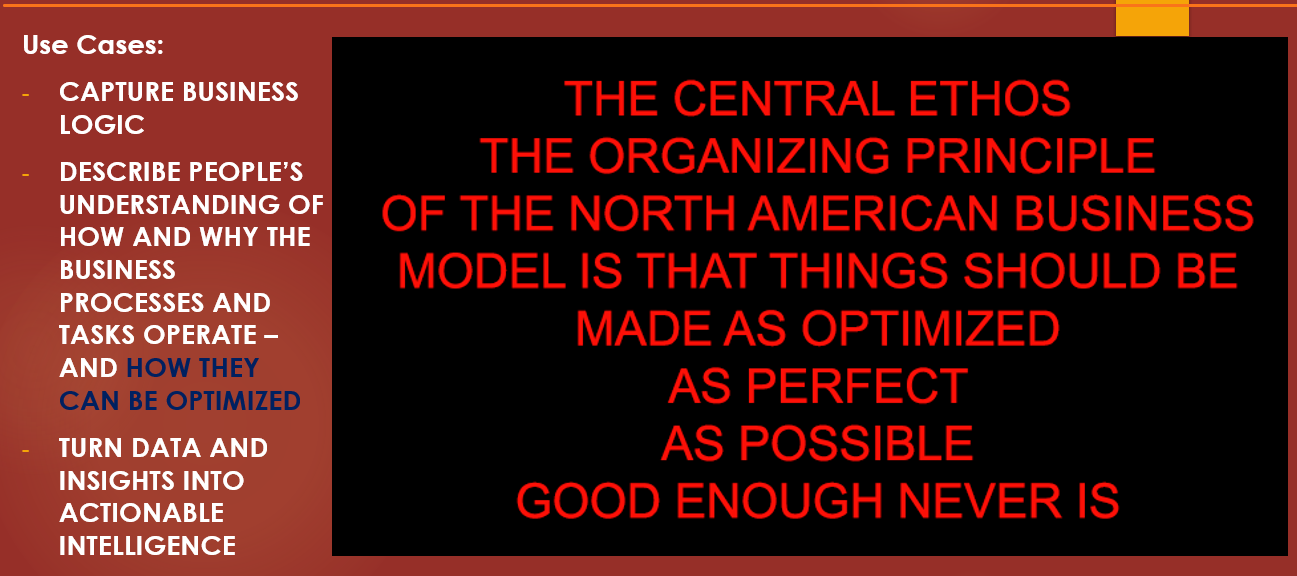
\includegraphics[scale=1.2]{use cases.png}


\subsection{Building the Tracability Matrix:}

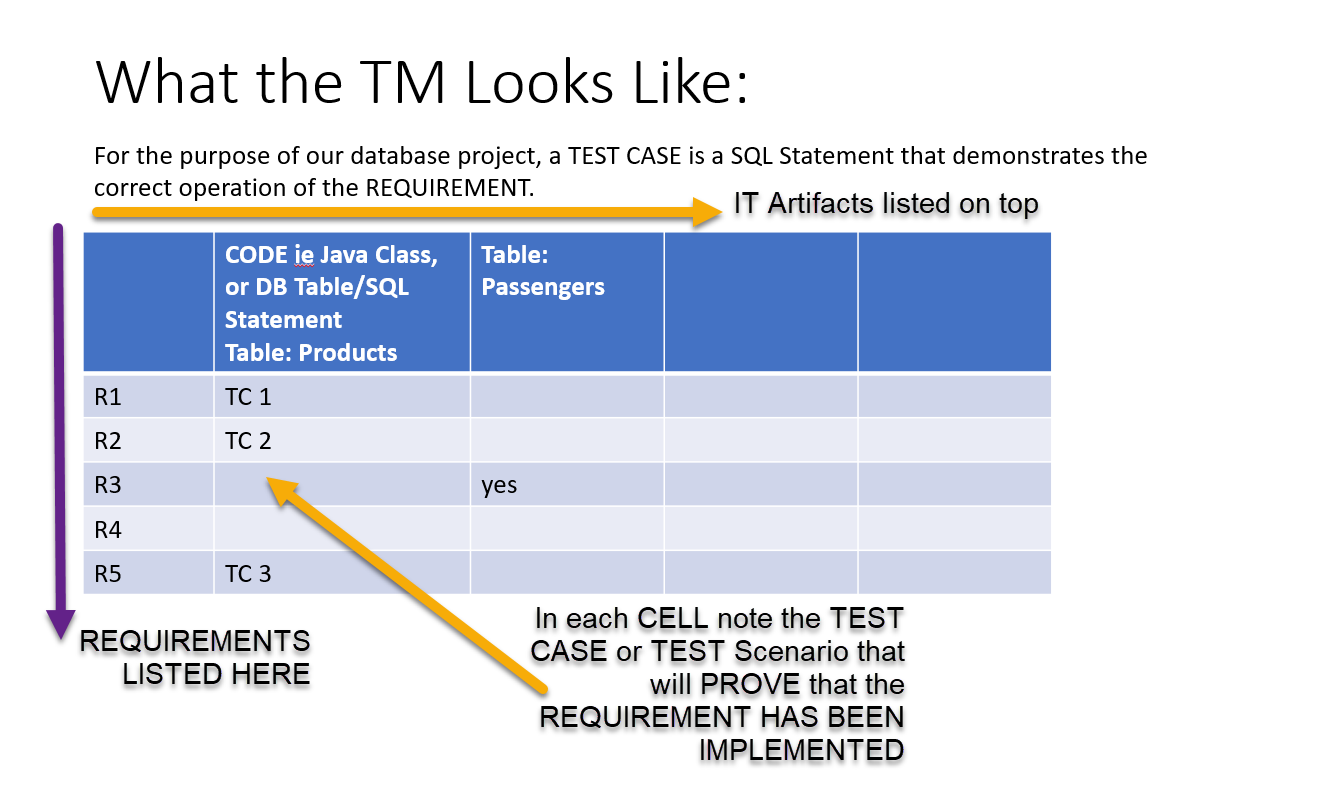
\includegraphics[scale=0.6]{images/TRACABILITYMATRIX.png}

\section{Requirements Analysis and Determination}

\begin{itemize}
    \item Writing a requirements document consists of interviewing stakeholders and user advocates. 
    \item A common practice is to ask them to write "user stories" - which just means that they will write down what ever they understand about how their job works.     
    \item Very few people really understand the details of the operation or job they're doing. The business analysts skill is to do the hard work of committing to diagrammatic communication (that's all UML diagrams are remember), and then sharing in joint application development sessions with the stakeholders and educating them until everyone can achieve a true consensus on what the system should do. 

    \item The Business Analyst may use UI Prototyping: Ask the users to draw out on paper Sketches of what the UI Screens should look with. The Screen is the User's Experience of the System.
    
\end{itemize}

The first and most critical skill for success as a business analyst is to commit to and work in a specific  industry domain, and apply yourself to becoming a subject management expert (SME).  
